\section{The \traceq Library}
\label{sec:mmc-traceq}

The \traceq library, one of the primary deliverables from this research, offers specialized Python profiling for detailed and accurate measurement of memory usage in Python programs.
Traditional methods for measuring memory, such as Docker container statistics or operating system (\ac{OS})-level queries, often miss Python-internal nuances or introduce significant overhead.
\traceq combines low-level Python profiling mechanisms with high-level system monitoring techniques, providing a targeted solution for memory-aware chunking applications and \ac{HPC} workflows.

\subsection{Motivation and Design Goals}
\label{sec:mmc-traceq-motivation}

Existing profiling tools commonly focus either on general-purpose \ac{CPU} profiling or offer only coarse-grained memory insights.
However, memory-aware chunking requires precise tracking of memory behavior over time.
The \traceq library meets these needs with the following key objectives:

\begin{itemize}
    \item \textbf{High-resolution memory tracing}: Accurately captures subtle, transient memory peaks essential for optimizing memory usage.
    \item \textbf{Minimal profiling overhead}: Ensures that measurements reflect actual application behavior, avoiding excessive performance penalties.
    \item \textbf{Cross-platform compatibility}: Works seamlessly across \ac{HPC} clusters, local environments, and Docker containers.
    \item \textbf{Ease of integration and usability}: Provides straightforward usage through command-line and Python \ac{API}s, enabling easy incorporation into existing workflows.
    \item \textbf{Avoiding intermediate state impact}: Prevents the profiler’s internal memory usage from significantly influencing measurement results, ensuring accurate reflection of the profiled application's true memory behavior.
\end{itemize}

By integrating Python-internal tools such as \texttt{tracemalloc} with \ac{OS}-level utilities like \texttt{psutil} and Docker or \ac{cgroup} statistics, \traceq provides a unified, reliable profiling mechanism suited to complex computational environments.

\subsection{Technical Implementation}
\label{sec:mmc-traceq-implementation}

\traceq leverages an adaptable backend architecture, allowing users to select among multiple profiling techniques to comprehensively measure memory usage:

\begin{itemize}
    \item \textbf{Python-internal tracing (\texttt{tracemalloc})}: Captures detailed memory allocation and deallocation patterns within Python’s managed heap, highlighting fine-grained memory dynamics.
    \item \textbf{System-level metrics (\texttt{psutil})}: Provides real-time monitoring of \ac{RSS} and virtual memory consumption, offering visibility into native extensions and non-Python memory allocations.
    \item \textbf{Kernel-level statistics (/proc)}: Integrates with Linux kernel metrics, essential for \ac{HPC} workflows and containerized applications.
    \item \textbf{Direct function-level tracing}: Identifies specific functions responsible for significant memory usage, enabling pinpoint accuracy in detecting memory-intensive code segments.
\end{itemize}

\traceq centralizes these measurement techniques through its core profiler engine, triggered via a simple \ac{CLI} or programmatically within Python scripts.
Configuration settings are flexible, supporting \ac{TOML} files, environment variables, and \ac{CLI} arguments, allowing precise control over profiling behavior.

\subsection{High-Level Architecture}
\label{sec:mmc-traceq-architecture}

The \traceq architecture comprises four main components:

\begin{enumerate}
    \item \textbf{\ac{CLI}}: Provides a user-friendly interface, parsing commands and initiating profiling tasks.
    \item \textbf{Configuration Module}: Manages profiling settings using a structured schema, consolidating input from various sources.
    \item \textbf{Core Profiler Engine}: Handles the execution of target Python scripts, orchestrating measurement intervals, trace collection, and data serialization.
    \item \textbf{Common Utilities}: Supplies shared functionalities such as logging, subprocess management, and configuration handling.
\end{enumerate}

\subsection{Profiling Workflow}
\label{sec:mmc-traceq-workflow}

When a profiling command such as \texttt{traceq profile script.py –metric memory,time} is executed, \traceq follows a structured workflow:

\begin{enumerate}
    \item Constructs instrumentation hooks based on user-selected metrics (memory, time).
    \item Instantiates a tracer object to schedule and manage periodic or event-based measurements.
    \item Launches the target Python script in a subprocess, embedding before-and-after execution hooks to capture precise snapshots of memory usage.
    \item Aggregates collected trace data, maintaining them in an internal memory buffer.
    \item Upon completion of the subprocess, consolidates collected traces into structured objects.
    \item Generates a comprehensive profiling report, including trace metadata and serialized measurement data.
\end{enumerate}

This workflow, as illustrated in Figure~\ref{fig:traceq_sequence}, ensures accurate tracking of memory dynamics, enabling insightful analysis of memory behavior in Python applications.

\begin{figure}[htbp]
    \centering
    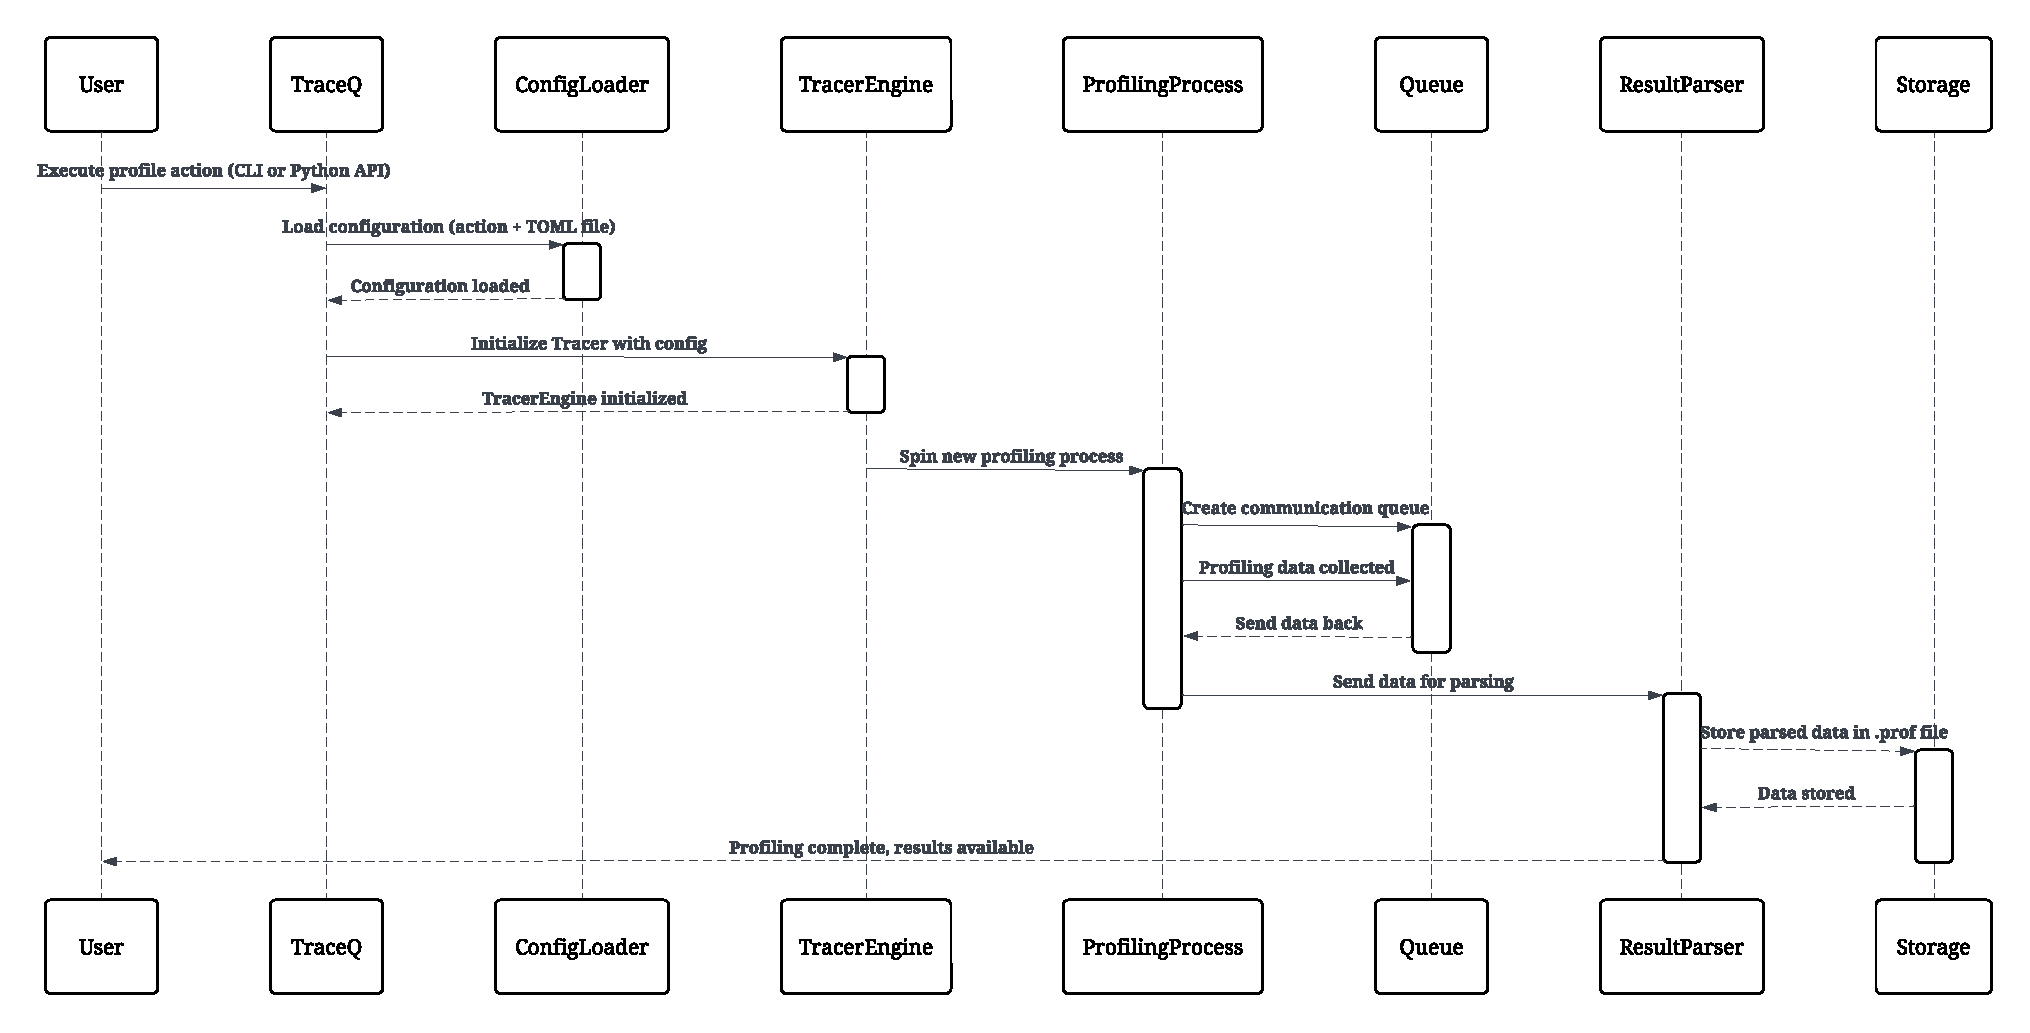
\includegraphics[width=\textwidth]{assets/images/04/traceq_sequence_diagram}
    \caption{
        This sequence diagram illustrates the overall flow and architecture of \traceq's profiling pipeline: it shows how a user-initiated profiling request is handled through a modular, asynchronous workflow—loading configuration, initializing the tracing engine, spawning a dedicated profiling process, and using an inter-process queue to collect, parse, and persist detailed profiling data—thereby enabling efficient, low-overhead memory tracing.%
    }
    \label{fig:traceq_sequence}
\end{figure}

\subsection{Usage Examples}
\label{sec:mmc-traceq-examples}

\textbf{Simple profiling example:}
\begin{verbatim}
traceq profile my_script.py –-enable-metric memory –-profiler-precision 1
\end{verbatim}

This command profiles memory usage with 100ms sampling intervals, generating detailed trace reports.

\textbf{Docker container profiling:}
\begin{verbatim}
docker run traceq profile main.py –-profiler-precision 4
\end{verbatim}

You can run within a Docker container, allowing for seamless integration into containerized workflows.

\textbf{Profiling with a decorator:}
\begin{verbatim}
from traceq import profile

@profile
def my_function():
    # Function code here
    pass
\end{verbatim}

This decorator enables profiling of specific functions, providing targeted insights into memory usage.

\subsection{Validation and Performance}
\label{sec:mmc-traceq-validation}

Validation studies detailed on Section~\ref{sec:mmc-recommended-strategy} confirm \traceq’s accuracy and low overhead.
Comparative benchmarking against \ac{OS}-level tools (Docker stats, \texttt{psutil}) demonstrates alignment within 2-3\% variance, accounting primarily for transient Python allocations and garbage collection effects.
Profiling overhead remains minimal, typically under 5\% for standard interval sampling, ensuring practical applicability for performance-sensitive scenarios.

In summary, the \traceq library provides a robust and precise solution for profiling memory usage, making it highly suitable for sophisticated computational workloads and memory-sensitive Python applications.